\documentclass[a4paper]{article}

\usepackage[english]{babel}
\usepackage[utf8]{inputenc}
\usepackage{etoolbox}
\usepackage{url}


\usepackage{tikz}
\usetikzlibrary{decorations.pathreplacing}

\title{audio-visual perception for recognition of human activities and object affordances for assistant robots.}


\begin{document}
	\maketitle


	\section{network}
	\label{sec:network}

		In order to perform the detection of human activities, we have planned to use three networks that will detect human sub-activities based on different inputs. The Three inputs we consider are :
		\begin{itemize}
			\item The visual context at the proximity of both hands.
			\item The global audio recording.
			\item The human skeleton position and speed informations.
		\end{itemize}
		These inputs are going to be processed differently. The first two inputs (visual and audio) are processed by Convolution Neural Network (CNN) and the third input, is processed thanks to hand-engineered features. These processing, results in three types of descriptors, possibly describing sub activities.

		\vskip .5cm
		\textbf{Visual CNN} \\

		The first processing channel we describe is the visual one. It's input is composed by a crop of the scene centered and normalized on the hand it's also a three dimensional array which contains an RGB-image. This image is processed by a CNN that has been trained on ImageNet\ref{sec:dataset}. At the end of the network, we aim at having descriptors indicating which sub-activities are being performed, such as having a phone on the hand.

		\vskip .5cm
		\textbf{Audio CNN}\\

		The second processing channel is based on the audio recording. We extract a sequence of ?? seconds and classify it thanks to a CNN. Here also, the network is trained on a third party dataset and is intended to retrieve relevant descriptors also helping at identifying sub-activities. We think here at recognizing people speaking or sounds being produced by object manipulation.

		\vskip .5cm
		\textbf{Skeleton pose} \\


		The third and last processing channel we use, before aggregating all the aforementioned channels, is the skeleton processing. For this channel, we are considering using a \textit{pose descriptor} as described in \cite{zanfir2013moving} resulting in spacio-temporal descriptors.

		
\newcommand*{\myBoxBlack}[6]{
	% 1 : p_x  --  4 : w_x
	% 2 : p_y  --  5 : w_y
	% 3 : p_z  --  6 : w_z
	\draw[black, fill=white] (#1,-#2,-#3) -- ++(-#4,0,0) -- ++(0,-#5,0) -- ++(#4,0,0) -- cycle;
	\draw[black, fill=white] (#1,-#2,-#3) -- ++(0,0,-#6) -- ++(0,-#5,0) -- ++(0,0,#6) -- cycle;
	\draw[black, fill=white] (#1,-#2,-#3) -- ++(-#4,0,0) -- ++(0,0,-#6) -- ++(#4,0,0) -- cycle;
}

\newcommand*{\myBoxBlackUnfilled}[6]{
	\draw[black] (#1,-#2,-#3) -- ++(-#4,0,0) -- ++(0,-#5,0) -- ++(#4,0,0) -- cycle;
	\draw[black] (#1,-#2,-#3) -- ++(0,0,-#6) -- ++(0,-#5,0) -- ++(0,0,#6) -- cycle;
	\draw[black] (#1,-#2,-#3) -- ++(-#4,0,0) -- ++(0,0,-#6) -- ++(#4,0,0) -- cycle;
}

\newcommand*{\myBoxGrey}[6]{
	\draw[black!60, fill=black!25] (#1,-#2,-#3) -- ++(-#4,0,0) -- ++(0,-#5,0) -- ++(#4,0,0) -- cycle;
	\draw[black!60, fill=black!25] (#1,-#2,-#3) -- ++(0,0,-#6) -- ++(0,-#5,0) -- ++(0,0,#6) -- cycle;
	\draw[black!60, fill=black!25] (#1,-#2,-#3) -- ++(-#4,0,0) -- ++(0,0,-#6) -- ++(#4,0,0) -- cycle;
}

	%%%%%%%%%%%%%%%%%%%%%%%%%%%%%%%%%%%%%%%%%%%% 
	%%% Draw the main framework
	%%%  With 3 processing thingy
	%%%  And a RNN
	%%%%%%%%%%%%%%%%%%%%%%%%%%%%%%%%%%%%%%%%%%%% 


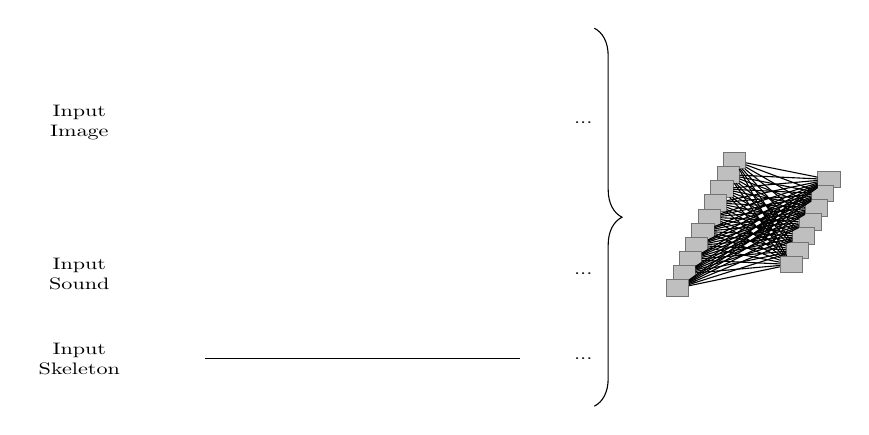
\begin{tikzpicture}[yscale=0.6, xscale=0.8, every node/.style={transform shape}]

	\node[text width=4em, text centered] (I-1) at (-2,-1) {Input Image};

	%%%%%%%%%%%%%%%%%%%%%%%%%%%%%%%%%%%%%%%%%%%% 
	%%% DRAW THE INPUT IMAGE
	%%%%%%%%%%%%%%%%%%%%%%%%%%%%%%%%%%%%%%%%%%%% 
	\myBoxGrey {0}{.2}{.2}{.3}{.5}{.5}
	\myBoxBlackUnfilled{0}{0}{0}{.3}{3}{3}

	%%% DRAW 1st ConvolutionLayer
	\myBoxBlack{2.5}{.25}{0}{1.5}{2.5}{2.5}
	\myBoxBlack{3}{.25}{0}{.3}{2.5}{2.5}
	\myBoxGrey{1.1}{.35}{0}{.05}{.1}{.1}

	%%% DRAW 2nd ConvolutionLayer
	\myBoxBlack{4.5}{.4}{0}{.7}{2}{2}
	\myBoxBlack{5}{.4}{0}{.3}{2}{2}

	%%%%%%%%%%%%%%%%%%%%%%%%%%%%%%%%%%%%%%%%%%%% 
	%%% draw split lines for Channels 
	% \foreach \channel in {1,...,15}{
	%     \draw[black,dashed] (2.5-\channel*.1,-.25,0) -- ++(0,-\cubey,0) ;
	%     \draw[black,dashed] (2.5-\channel*.1,-.25,0) -- ++(0,0,-\cubez) ;
	% }

	\node[text width=4em, text centered] (I-1) at (6,-1) {...};


	%%%%%%%%%%%%%%%%%%%%%%%%%%%%%%%%%%%%%%%%%%%% 
	%%% DRAW THE INPUT SOUND
	%%%%%%%%%%%%%%%%%%%%%%%%%%%%%%%%%%%%%%%%%%%% 
	\pgfmathsetmacro{\yPading}{4.2}
	\node[text width=4em, text centered] (I-1) at (-2,-\yPading) {Input Sound};
	\myBoxGrey {0}{.1-\yPading}{.2}{.3}{.3}{.5}
	\myBoxBlackUnfilled{0}{0-\yPading}{0}{.3}{.5}{3}
	\myBoxBlack{2.5}{0-\yPading}{0}{1.5}{.5}{2.5}
	\myBoxBlack{3}{0-\yPading}{0}{.3}{.5}{2.5}
	\myBoxGrey{1.1}{0-\yPading}{0}{.05}{.3}{.1}
	\myBoxBlack{4.5}{0-\yPading}{0}{.7}{.5}{2}
	\myBoxBlack{5}{0-\yPading}{0}{.3}{.5}{2}
	\node[text width=4em, text centered] (I-1) at (6,-\yPading) {...};

	%%%%%%%%%%%%%%%%%%%%%%%%%%%%%%%%%%%%%%%%%%%% 
	%%% DRAW THE INPUT SKELETON
	%%%%%%%%%%%%%%%%%%%%%%%%%%%%%%%%%%%%%%%%%%%% 
	\pgfmathsetmacro{\yPading}{6}
	\node[text width=4em, text centered] (I-1) at (-2,-\yPading) {Input Skeleton};
	\draw (0,-\yPading) -- (5,-\yPading);
	\node[text width=4em, text centered] (I-1) at (6,-\yPading) {...};


	\draw [decorate,decoration={brace,amplitude=10pt,mirror,raise=4pt},yshift=0pt] (6,-7) -- (6,1) ;


	%%%%%%%%%%%%%%%%%%%%%%%%%%%%%%%%%%%%%%%%%%%% 
	%%% DRAW THE RNN
	%%%%%%%%%%%%%%%%%%%%%%%%%%%%%%%%%%%%%%%%%%%% 
	\tikzstyle{smallneuron}=[rectangle,fill=black!25,minimum size=10pt,inner sep=0pt, line width=0.1mm, draw=black!55]

	\def\xPos{6.5}
	\def\yPos{-2}
   	\foreach \name / \y in {1,...,10}
        \path[yshift=0.5cm] node[smallneuron] (RNN1-\name) at (\xPos+10*0.2-\y*0.1, \yPos -\y*0.3) {};

    \def\xPos{8}
    \def\yPos{-2.4}
   	\foreach \name / \y in {1,...,7}
        \path[yshift=0.5cm] node[smallneuron] (RNN2-\name) at (\xPos+10*0.2-\y*0.1, \yPos -\y*0.3) {};

    \foreach \source in {1,...,10}
        \foreach \dest in {1,...,7}
            \path (RNN1-\source) edge (RNN2-\dest);

\end{tikzpicture}


	% \begin{figure}
	% 	\centering
	% 	\def\layersep{1.5cm}
	% 	\begin{tikzpicture}[shorten >=1pt,->,draw=black!50, node distance=\layersep, yscale=1]
	% 	    \tikzstyle{every pin edge}=[<-,shorten <=1pt]
	% 	    \tikzstyle{neuron}=[rectangle,fill=black!25,minimum size=17pt,inner sep=0pt, line width=0.1mm, draw=black!55]
	% 	    \tikzstyle{smallneuron}=[rectangle,fill=black!25,minimum size=10pt,inner sep=0pt, line width=0.1mm, draw=black!55]
	% 	    \tikzstyle{input}=[rectangle,fill=black!5,minimum size=25pt,inner sep=0pt, line width=0.1mm, draw=black!55]
	% 	    \tikzstyle{annot} = [text width=4em, text centered]


	% 	    %%%%%%%%%%%%%%%%%%%%%%%%%%%%%%%%%%%%%%%%%%%% 
	% 	    %%% DRAW THE SQUARES
	% 	    %%%%%%%%%%%%%%%%%%%%%%%%%%%%%%%%%%%%%%%%%%%%
		    
	% 	    \node[input] (I-1) at (0,-1.25) {$x_{i1}$};

	% 	    \foreach \name / \y in {1,...,10}
	% 	        \path[yshift=0.5cm] node[smallneuron] (H1-\name) at (\layersep+10*0.2cm-\y*0.2cm, -\y*0.3 cm) {};

	% 		\foreach \name / \y in {1,...,7}
	% 	        \path[yshift=1.5cm] node[neuron] (H2-\name) at (\layersep*3+7*0.2cm-\y*0.2cm,-\y*0.3 cm -1.25cm) {};   

	       	
	% 	    \node[neuron,pin={[pin edge={->}]right:$p_{i1}$}, right of=H2-3] (O-1) {};
	% 	    \node[neuron,pin={[pin edge={->}]right:$p_{i2}$}, right of=H2-5] (O-2) {};

	% 	    %%%%%%%%%%%%%%%%%%%%%%%%%%%%%%%%%%%%%%%%%%%% 
	% 	    %%% DRAW THE PATHS
	% 	    %%%%%%%%%%%%%%%%%%%%%%%%%%%%%%%%%%%%%%%%%%%%
	% 	    \foreach \source in {1}
	% 	        \foreach \dest in {1,...,10}
	% 	            \path (I-\source) edge (H1-\dest);

	% 	    \foreach \source in {1,...,10}
	% 	        \foreach \dest in {1,...,7}
	% 	            \path (H1-\source) edge (H2-\dest);

	% 	    \foreach \source in {1,...,7}
	% 	    	\foreach \dest in {1,...,2}
	% 		        \path (H2-\source) edge (O-\dest);

	% 	    % Annotate the layers
	% 	    \node[annot,above of=H2-1, node distance=1cm] (hl) {Hidden layer 2};
	% 	    \node[annot,left of=hl] (hl1) {Hidden layer 1};
	% 	    \node[annot,left of=hl1] {Input layer};
	% 	    \node[annot,right of=hl] {Output layer};
	% 	\end{tikzpicture}
	% 	\caption{Feed-forward neural-network with two hidden layers}
	% 	\label{fig:feed_forward}
	% \end{figure}
	
	\section{Dataset}
	\label{sec:dataset}

		In this section we present the different datasets used to train the four different parts of our network. Hence, we present the dataset used for image processing followed by the dataset used for sound processing, then the one for skeleton processing and, finally, the dataset that'll be used for training the RNN. The intuition beneath such needs is presented in section \ref{sec:network}.

		\vskip .5cm
		\textbf{Image dataset} \\
		\label{sub:image_dataset}

		ImageNet\cite{ILSVRC15} is a reference dataset in image processing. Many famous CNN architecture are based on this dataset such as AlexNet, GoogLeNet or NiNet. A contest is based on this dataset and the 2015'th edition of this contest has more than $450000$ images of mean resolution of $482*415$ pixels organized in 200 labeled categories (such as airplane, ant, antelope, apple and axe) for object detection in images \footnote{\url{http://www.image-net.org/challenges/LSVRC/2014/}}.
		Though ImageNet 2015's contest doesn't include neither phones nor book, we can append them to our dataset thanks to the ImageNet main dataset consisting of over $14*10^6$ images \footnote{\url{http://www.image-net.org/synset?wnid=n02992529#}}.
		We use this dataset to train our 2D image convolution neural network seen on section\ref{sec:network}.

		For later uses, we might consider the video dataset consisting of 401 categories for scene classification also present on the ImageNet 2015's contest.

		\vskip .5cm
		\textbf{Audio dataset} \\
		\label{sub:audio_dataset}



		\vskip .5cm
		\textbf{skeleton dataset} \\
		\label{sub:skeleton_dataset}


	\section{Testing}
	\label{sec:testing}
	
		For testing purposes, we've build three datasets. We believe that the evaluation of human action recognition is increasingly harder on each of these datasets. 


		\subsection{First set}
		\label{sub:first_set}
		
			The first set we recorded captured 5 actions : sitting down, reading, calling, drinking and sitting up. Each of these actions were captured based on the following scenario:

			There is a camera behind a blank table seeing both the table and a chair behind it. A man comes in and sit on the chair. He'll then perform a set of three (non-sitting) actions. First, he'll read a book, secondly, he'll answer a phone call and thirdly he'll drink the content of a mug. The setup is such as the table is clear at the beginning of these action. When an action begins, the man puts the object he'll use on the table, then he uses it (reading, calling or drinking) and, at the end of the action, he puts back the object on the table before clearing it off. Once these three actions are performed, the man leaves the room. To see a video extract of this dataset you can watch a Youtube video\footnote{\url{https://www.youtube.com/watch?v=VvPMcFAKO3U}}.
			
			As a technical matter, we've captured a 340p RGBD video stream at 15 fps and the audio stream at 28kHz. The depth image we use is the Xtion's one.






	


	\bibliographystyle{plain}
	\bibliography{papers}


\end{document}